\title{\bf{Comparrison of Backpropogation, Genetic method, and Decision Tree
method for Diabetes Diagnosis Prediction}}
\author{}
\date{\today}

\documentclass[12pt]{article}
\usepackage{graphicx}
\usepackage{hyperref}
\graphicspath{ {./images/} }
\begin{document}
\maketitle

\section{Introduction}
    \subsection{Project Motivation}
        The motivation of this project originated from curiosity about the nature of neural 
        networks and the efficiency of the different methods used to train them.
    \subsection{Aims and Objectives}
        The objective of the project is to test the methods of backpropogation, genetic 
        algorithms, and decision trees on a diabetes diagnosis training set.
    \subsection{Report Structure}
\section{Background and History of the Study}
    Originally only concentrating on neural networks that utilize decision trees, 
    the scope of the project has grown to include the learning methods of backpropogation and 
    genetic algorithms as time has permitted.  Neural networks produce result through the many interactions 
    between its neurons.  The neurons are organized in layers; The first layer is the input layer, 
    where data is first given to the network.  The last layer is the output layer, which takes input 
    from other neurons and outputs the result of the network.  Between these layers are zero or more 
    hidden layers.  They function the same as the output layer, taking input from the layer before it 
    and producing an output.
\section{Implementation}
    The first steps to conducting the experiment were to craft each of the different neural networks. 
    \subsection{Backpropogation} 
        The backpropogation network was first, originally utilizing a graph data structure for its 
        implementation.  The network was first ordered by layers, with the nodes of the graph (neurons) 
        being organized by layer in arrays, with each node being connected to every node in the layer after it.  
        Nodes fired after all of the nodes connecting to it had already fired, with the output layer yielding a result right after the 
        input layer was set with a sample to train on.
        \begin{figure}[h]
            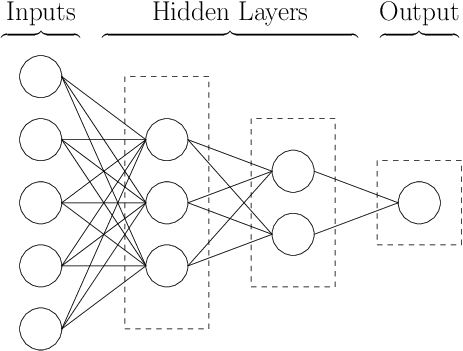
\includegraphics[scale=.3]{nnDiagram.png}
            \centering
            \caption{Example of a Neural Network}
        \end{figure}
        Output from these neurons is produced by taking the sum of all its inputs (\(I_i\)), each multiplied by a weight (\(W_i\)), 
        and subtracting the neuron's bias (\(b\)).  The result of this summation is then passed into the activation function to produce 
        the final output of the neuron. The activation function scales the summation to be between zero and one.  The sigmoid (\(\sigma\))function
        was used in this experiment.
        \begin{equation}\label{inputSum}
            Y = \sigma[\sum_{i=1}^{n} (I_i W_i) - b] 
        \end{equation}
        One of the most popular methods of training neural networks is through backpropogation.  
        In this method, the network is fed how different each layer's output was from the correct output, 
        starting at the output layer and ending at the first hidden layer.

        The error between the expected output and the observed output (\(e\)) is calculated by taking their difference.
        The error gradient of the neuron, used to calculate the change in each weight, is calculated by using a formula similar
        to \ref{inputSum} but using the derivative of \(\sigma\) instead of \(\sigma\) itself multiplied by the error (\(e\)).
        \begin{equation}\label{errGradient}
            \delta = \frac{d\sigma}{dx}[\sum_{i=1}^{n} (I_i W_i) - b]*e
        \end{equation}
        The change for each weight (\(\Delta W_i\)) in the output nodes is calculated by multiplying the error gradient (\(\delta\)),
        a learning rate constant (\(\alpha\)), and the previous output (\(Y_p\)) of the node together.
        \begin{equation}\label{outputWeightDelta}
            \Delta Y = \delta*\alpha*Y_p
        \end{equation}
        For the hidden layers, then change in their weights are similar.  Instead of the error of the output nodes, however,
        the summation of each error gradient of the nodes in the previous layer (\(\delta_j\) for node \(j\) in the previous layer) 
        multiplied by their weights for the current node (\(W_j\)).
        \begin{equation}\label{hiddenWeightDelta}
            \delta = \frac{d\sigma}{dx}[\sum_{i=1}^{n} (I_i W_i) - b]*\sum_{j=1}^{n_p} (\delta_j W_j)
        \end{equation}
        When this process is repeated for many epochs over one data set, the output of the network becomes more
        tuned to the desired result.
    \subsection{Genetic Algorithm}
        Genetic algorithms are quite different from backpropogation, utilizing trends within nature as inspiration.
        The training begins with a population of randomly generated individuals.  Each indivudual is composed of a genome which 
        describes every weight and bias of every neuron within a neural network.  Each gene within that genome represents
        the set of all weights (one from each node in layer \(i\)) relating to the connections of one node in layer \(i-1\).

        As the training begins, each member of the polulation has its fitness evaluated.  The evaluation function for this project
        is the reciprocal of the loss function, \(fitness(memberId) = \frac{1}{loss(memberId)}\).  Two parents from the population
        are then selected using the roulette wheel method, where parents are randomly chosen, biased twoard parents with high fittness scores.
        The genomes of the parents are crossed between two new children.  A point on the genome is randomly chosen (\(p\)) where
        child genes are composed of correcponding parent genes for the section up to \(p\) then composed of the oppisite parent after \(p\).
        \begin{figure}[h]
            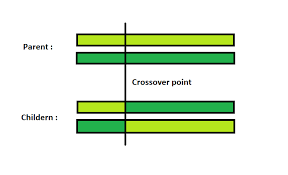
\includegraphics[scale=.5]{crossover.png}
            \centering
            \caption{Illustration of crossover}
        \end{figure}
        This ensures that there is a good mix between the characteristics of the parents passed down to the children.

        Each child may then undergo a mutation, where an individual gene is mutated to a random value.  This serves the
        purpose of guiding genes out of local maximums (genes that evolve to do well for a specific subset of samples, but
        not the samples as a whole).
        
        This cycle continues until the amount of children produces equals the size of the original population.  The population
        is then replaced with the children.  This represents on generation of the neural network.
        When this process is repeated for many epochs over one data set, the output of the network becomes more
        tuned to the desired result.
        \subsection{Decision Tree}
            %TODO decision tree section%
\section{Experimental Approach}
    \subsection{Data Set and Preparation}
        The data set used for this project is from the Vanderbilt University Department of Biostatics and contains
        the testing parameters and results of 390 African American participants from central Virginia.
        The parameters of the dataset are comprised of the patient's cholesterol, blood glucode levels, high-density lipoprotein (HDL)
        or "good" cholesterol, the ratio of HDL cholesterol to total cholesterol, age, gender, height, weight, body mass index (BMI),
        systolic blood pressure, and diastolic blood pressure.  The entries in the dataset are categorized into two groups, those that
        were diagnosed with diabestes and those who were not.  For this experiment, the height and weight parameters were exclused
        as they were redundant with BMI.  The cholesterol ratio parameter was also omitted for redundancy to the other cholesterol parameters.

        Before usage in training, the data set was first normalized.  When a data set is normalized, all of its values are scaled
        between zero and one.  Zero is set as the lowest value a parameter can take

        %TODO mention normalization as preparation%
\section{Results and Discussion}

\section{Conclusions}

\begin{thebibliography}{100}
    %(Fig. 1) \url{https://www.researchgate.net/figure/Simple-neural-network-diagram_fig1_332158639}
    %(Fig. 2) \url{https://www.geeksforgeeks.org/crossover-in-genetic-algorithm/}
    %Diabetes data set https://hbiostat.org/data/%
\end{thebibliography}

\end{document}